\documentclass[]{book}
\usepackage{lmodern}
\usepackage{amssymb,amsmath}
\usepackage{ifxetex,ifluatex}
\usepackage{fixltx2e} % provides \textsubscript
\ifnum 0\ifxetex 1\fi\ifluatex 1\fi=0 % if pdftex
  \usepackage[T1]{fontenc}
  \usepackage[utf8]{inputenc}
\else % if luatex or xelatex
  \ifxetex
    \usepackage{mathspec}
  \else
    \usepackage{fontspec}
  \fi
  \defaultfontfeatures{Ligatures=TeX,Scale=MatchLowercase}
\fi
% use upquote if available, for straight quotes in verbatim environments
\IfFileExists{upquote.sty}{\usepackage{upquote}}{}
% use microtype if available
\IfFileExists{microtype.sty}{%
\usepackage[]{microtype}
\UseMicrotypeSet[protrusion]{basicmath} % disable protrusion for tt fonts
}{}
\PassOptionsToPackage{hyphens}{url} % url is loaded by hyperref
\usepackage[unicode=true]{hyperref}
\hypersetup{
            pdftitle={An Exam P Study Guide},
            pdfauthor={Actuary Helper},
            pdfborder={0 0 0},
            breaklinks=true}
\urlstyle{same}  % don't use monospace font for urls
\usepackage{natbib}
\bibliographystyle{apalike}
\usepackage{color}
\usepackage{fancyvrb}
\newcommand{\VerbBar}{|}
\newcommand{\VERB}{\Verb[commandchars=\\\{\}]}
\DefineVerbatimEnvironment{Highlighting}{Verbatim}{commandchars=\\\{\}}
% Add ',fontsize=\small' for more characters per line
\usepackage{framed}
\definecolor{shadecolor}{RGB}{248,248,248}
\newenvironment{Shaded}{\begin{snugshade}}{\end{snugshade}}
\newcommand{\KeywordTok}[1]{\textcolor[rgb]{0.13,0.29,0.53}{\textbf{#1}}}
\newcommand{\DataTypeTok}[1]{\textcolor[rgb]{0.13,0.29,0.53}{#1}}
\newcommand{\DecValTok}[1]{\textcolor[rgb]{0.00,0.00,0.81}{#1}}
\newcommand{\BaseNTok}[1]{\textcolor[rgb]{0.00,0.00,0.81}{#1}}
\newcommand{\FloatTok}[1]{\textcolor[rgb]{0.00,0.00,0.81}{#1}}
\newcommand{\ConstantTok}[1]{\textcolor[rgb]{0.00,0.00,0.00}{#1}}
\newcommand{\CharTok}[1]{\textcolor[rgb]{0.31,0.60,0.02}{#1}}
\newcommand{\SpecialCharTok}[1]{\textcolor[rgb]{0.00,0.00,0.00}{#1}}
\newcommand{\StringTok}[1]{\textcolor[rgb]{0.31,0.60,0.02}{#1}}
\newcommand{\VerbatimStringTok}[1]{\textcolor[rgb]{0.31,0.60,0.02}{#1}}
\newcommand{\SpecialStringTok}[1]{\textcolor[rgb]{0.31,0.60,0.02}{#1}}
\newcommand{\ImportTok}[1]{#1}
\newcommand{\CommentTok}[1]{\textcolor[rgb]{0.56,0.35,0.01}{\textit{#1}}}
\newcommand{\DocumentationTok}[1]{\textcolor[rgb]{0.56,0.35,0.01}{\textbf{\textit{#1}}}}
\newcommand{\AnnotationTok}[1]{\textcolor[rgb]{0.56,0.35,0.01}{\textbf{\textit{#1}}}}
\newcommand{\CommentVarTok}[1]{\textcolor[rgb]{0.56,0.35,0.01}{\textbf{\textit{#1}}}}
\newcommand{\OtherTok}[1]{\textcolor[rgb]{0.56,0.35,0.01}{#1}}
\newcommand{\FunctionTok}[1]{\textcolor[rgb]{0.00,0.00,0.00}{#1}}
\newcommand{\VariableTok}[1]{\textcolor[rgb]{0.00,0.00,0.00}{#1}}
\newcommand{\ControlFlowTok}[1]{\textcolor[rgb]{0.13,0.29,0.53}{\textbf{#1}}}
\newcommand{\OperatorTok}[1]{\textcolor[rgb]{0.81,0.36,0.00}{\textbf{#1}}}
\newcommand{\BuiltInTok}[1]{#1}
\newcommand{\ExtensionTok}[1]{#1}
\newcommand{\PreprocessorTok}[1]{\textcolor[rgb]{0.56,0.35,0.01}{\textit{#1}}}
\newcommand{\AttributeTok}[1]{\textcolor[rgb]{0.77,0.63,0.00}{#1}}
\newcommand{\RegionMarkerTok}[1]{#1}
\newcommand{\InformationTok}[1]{\textcolor[rgb]{0.56,0.35,0.01}{\textbf{\textit{#1}}}}
\newcommand{\WarningTok}[1]{\textcolor[rgb]{0.56,0.35,0.01}{\textbf{\textit{#1}}}}
\newcommand{\AlertTok}[1]{\textcolor[rgb]{0.94,0.16,0.16}{#1}}
\newcommand{\ErrorTok}[1]{\textcolor[rgb]{0.64,0.00,0.00}{\textbf{#1}}}
\newcommand{\NormalTok}[1]{#1}
\usepackage{longtable,booktabs}
% Fix footnotes in tables (requires footnote package)
\IfFileExists{footnote.sty}{\usepackage{footnote}\makesavenoteenv{long table}}{}
\usepackage{graphicx,grffile}
\makeatletter
\def\maxwidth{\ifdim\Gin@nat@width>\linewidth\linewidth\else\Gin@nat@width\fi}
\def\maxheight{\ifdim\Gin@nat@height>\textheight\textheight\else\Gin@nat@height\fi}
\makeatother
% Scale images if necessary, so that they will not overflow the page
% margins by default, and it is still possible to overwrite the defaults
% using explicit options in \includegraphics[width, height, ...]{}
\setkeys{Gin}{width=\maxwidth,height=\maxheight,keepaspectratio}
\IfFileExists{parskip.sty}{%
\usepackage{parskip}
}{% else
\setlength{\parindent}{0pt}
\setlength{\parskip}{6pt plus 2pt minus 1pt}
}
\setlength{\emergencystretch}{3em}  % prevent overfull lines
\providecommand{\tightlist}{%
  \setlength{\itemsep}{0pt}\setlength{\parskip}{0pt}}
\setcounter{secnumdepth}{5}
% Redefines (sub)paragraphs to behave more like sections
\ifx\paragraph\undefined\else
\let\oldparagraph\paragraph
\renewcommand{\paragraph}[1]{\oldparagraph{#1}\mbox{}}
\fi
\ifx\subparagraph\undefined\else
\let\oldsubparagraph\subparagraph
\renewcommand{\subparagraph}[1]{\oldsubparagraph{#1}\mbox{}}
\fi

% set default figure placement to htbp
\makeatletter
\def\fps@figure{htbp}
\makeatother

\usepackage{booktabs}
\usepackage{amsthm}
\makeatletter
\def\thm@space@setup{%
  \thm@preskip=8pt plus 2pt minus 4pt
  \thm@postskip=\thm@preskip
}
\makeatother

\title{An Exam P Study Guide}
\author{Actuary Helper}
\date{2019-12-22}

\begin{document}
\maketitle

{
\setcounter{tocdepth}{1}
\tableofcontents
}
\chapter{An Introduction to Set
Theory}\label{an-introduction-to-set-theory}

\section{Defining Sets}\label{defining-sets}

Sets are collections of objects. Usually objects are placed inside curly
braces and separated by commas. Here is the set with the numbers 1 and
2. We often give sets a name. This set is named ``A''. \[A=\{1,2\}\]

Objects inside the curly braces are called elements of the set. There is
a special character that means ``is an element of''. Using our notation
we can say that 1 is an element of A. \[1 \in A\]

We can also say that 3 is not an element of A by drawing a slash through
our symbol. \[3 \not\in A\] We can define sets in a something called
set-builder notation. Set builder notation is useful for infinite sets
or sets that are hard to enumerate. Below are some examples.

We can define the even numbers as
\(\{x | x \ is \  an \  even \ number\}\)

We can define hands of cards as
\(\{x | x \ is \  a \ 5 \ element \ subset \ of \ a \ deck \ of \ cards\}\)

To read set builder notation we translate the ``\textbar{}'' as
``where''. So the real numbers are ``the set of x where x is a real
number''.

\section{Set Equality and Subsets}\label{set-equality-and-subsets}

Sets are equal when they have the same elements. This means order
doesn't matter in sets, \(\{1,2\} = \{2,1\}\) because they have the same
elements. Also, \(\{1,1,2\} = \{1,2\}\) and we say that sets don't have
duplicate elements because duplicate elements have no purpose.

A set is a subset of another set when it fits inside of it. There is a
symbol that looks like \(\leq\) that means ``is a subset of''. For
example \(\{1,2\} \subseteq \{1,2,3\}\). It is also true that any set is
a subset of itself, so \(\{1,2\} \subseteq \{1,2\}\). In more precise
terms \(A \subseteq B\) if and only if every element of A is also an
element of B.

A common technique to prove that two sets are equal is to show that
\(A \subseteq B\) and \$ B \subseteq A\$. This means there is no element
in either set that does not belong to the other and the sets are equal.

\section{Set Operations and Venn
Diagrams}\label{set-operations-and-venn-diagrams}

Just like you can add numbers together to make a new number, you can
combine sets and make a new set. Let's define some sets.

\[S = \{1,2,3,4,5,6,7,8,9,10\} \\
 A = \{1,3,5,7\} \\
 B = \{2,3,4,5\}\]

\subsection{Venn Diagram}\label{venn-diagram}

There is a visual representation of sets called a Venn Diagram. In a
Venn Diagram each set is represented by a circle. The sample space is
usually represented by a large box that the circles are inside of.

\begin{figure}
\centering
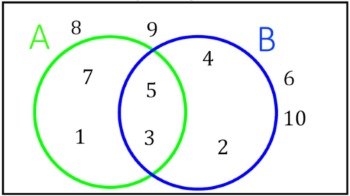
\includegraphics{Pictures/01-Sets/Venn.PNG}
\caption{}
\end{figure}

\subsection{Union}\label{union}

An element is in the union of A and B if it is in A, B, or A and B. The
notation for this operation is \(A \cup B\) and it is pronounced ``A
union B''. Here is the set that results from this union: \$ A \cup B =
\{1,2,3,4,5,7\}\$

\begin{figure}
\centering
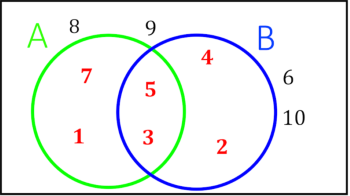
\includegraphics{Pictures/01-Sets/AUB.PNG}
\caption{}
\end{figure}

\subsection{Intersection}\label{intersection}

An element is in the intersection of A and B if it is in A and B. The
notation for this operation is \$ A \cap B\$ and it is pronounced ``A
intersect B''. Here is the set that results from this intersection:
\(A \cap B = \{3,5\}\)

\begin{figure}
\centering
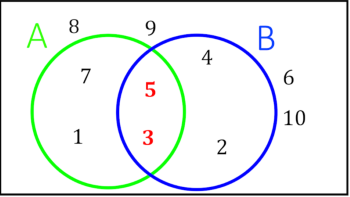
\includegraphics{Pictures/01-Sets/AcapB.PNG}
\caption{}
\end{figure}

\subsection{Complement}\label{complement}

An element is in the complement of A if it is not in A, but is in the
sample space. The notation for the complement of A is \(A^C\) and is
pronounced ``A complement'' or ``the complement of A''. Here is the
result of taking the complement of A: \(A^C = \{2,4,6,8,9,10\}\). Note
that in general \((A^C)^C = A\).

\begin{figure}
\centering
\includegraphics{Pictures/01-Sets/A\^{}C.PNG}
\caption{}
\end{figure}

\subsection{Set Difference}\label{set-difference}

The set difference of A and B elements that are in A but not in B. The
notation is either \(A \backslash B\) or \(A - B\) and is pronounced ``A
minus B''. Here is the result of this set difference:
\(A - B = \{7,1\}\). It is worth noting that \(A-B=A \cap B^C\) because
the elements are in A and they are not in B.

\begin{figure}
\centering
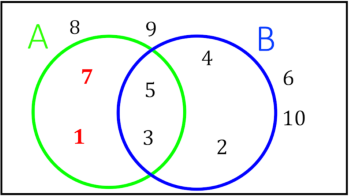
\includegraphics{Pictures/01-Sets/A-B.PNG}
\caption{}
\end{figure}

\section{Special Sets and Identities}\label{special-sets-and-identities}

\subsection{Sample Space and Empty
Set}\label{sample-space-and-empty-set}

The sample space is a type of special set because all other sets are
subset of it. This leads to some commonsensical identities like
\(A \cup S = S\) and \(A \cap S = A\). There is another special set
called the empty set. This set has no elements. We could write it as
\(\{\}\) but the common way to write this is \(\emptyset\). Some
properties of the empty set are \(A \cup \emptyset = A\) and
\(A \cap \emptyset = \emptyset\). It is also true that
\(\emptyset^C = S\) and \$ S\^{}C = \emptyset\$.

\subsection{De Morgan's Laws}\label{de-morgans-laws}

De Morgan's laws are formulas for the complement of a union or
intersection of sets. \[(A \cap B)^C = A^C \cup B^C \\
 (A \cup B)^C = A^C \cap B^C\] One way of memorizing these formulas is
that you bring the complement inside the parentheses to both sets and
flip the union or intersection upside down.

Let's see if these laws make any sense. Let \(T\) be the set of tennis
players and \(H\) be the set of hockey players. \((T \cap H)^C\) is the
set of people that don't play both tennis and hockey. \(T^C \cup H^C\)
is people that don't play tennis or they don't play hockey.If I don't
play both sports then I either don't play tennis or I don't play hockey,
so \((T \cap H)^C \subseteq T^C \cup H^C\). If I don't play tennis or I
don't play hockey then it is true that I don't play both sports, so
\(T^C \cup H^C \subseteq (T \cap H)^C\). This means that the sets are
equal, ponder this for some time. A similar argument can be made for the
complement of the union. If this is not convincing spend some time with
a Venn diagram and see if you can get it to make sense.

\subsection{3 or More Sets}\label{or-more-sets}

\subsubsection{Associativity}\label{associativity}

Just like you can add more than two numbers together you can take the
intersection or union of more than two sets. For example
\(\{1,2\} \cap \{2,3\} \cap \{3,4\} = \emptyset\). There are no elements
in the intersection of these three sets because no number appears in all
three sets, so this is the empty set. Intersections are associative,
meaning \((A \cap B) \cap C= A \cap (B \cap C)\), so it doesn't matter
what order you take a group of intersections in. Unions are also
associative, \((A \cup B) \cup C= A \cup (B \cup C)\).

\subsubsection{Messy Venn Diagrams}\label{messy-venn-diagrams}

You can draw a Venn diagram for three sets with three circles. It gets a
little complicated. I wouldn't bother drawing a Venn diagram for 4 sets.

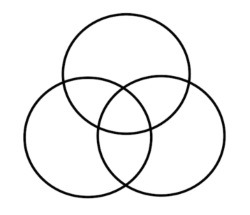
\includegraphics{Pictures/01-Sets/Venn3.PNG}
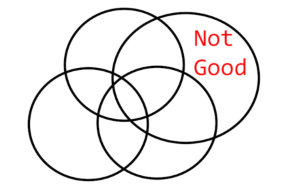
\includegraphics{Pictures/01-Sets/Venn4.PNG}

\subsubsection{Distributive Property}\label{distributive-property}

If you mix together unions and intersections in an expression it isn't
associative. Can you think of an example?
\[A \cap (B \cup C) \not= (A \cap B) \cup C\] There are distributive
formulas for situations like this.
\[ A \cap (B \cup C) = (A \cap B) \cup (A \cap C) \\
 A \cup (B \cap C) = (A \cup B) \cap (A \cup C)\] Because of this it is
said that intersection distributes over unions, and that unions
distribute across intersections. It is easier to remember these
distributive formulas by comparing them to the way multiplication
distributes over addition. \(a(b+c)=ab+ac\). Just pretend that the
multiplication is an intersection and the addition is a union.

\chapter{Introduction}\label{intro}

You can label chapter and section titles using \texttt{\{\#label\}}
after them, e.g., we can reference Chapter \ref{intro}. If you do not
manually label them, there will be automatic labels anyway, e.g.,
Chapter \ref{methods}.

Figures and tables with captions will be placed in \texttt{figure} and
\texttt{table} environments, respectively.

\begin{Shaded}
\begin{Highlighting}[]
\KeywordTok{par}\NormalTok{(}\DataTypeTok{mar =} \KeywordTok{c}\NormalTok{(}\DecValTok{4}\NormalTok{, }\DecValTok{4}\NormalTok{, .}\DecValTok{1}\NormalTok{, .}\DecValTok{1}\NormalTok{))}
\KeywordTok{plot}\NormalTok{(pressure, }\DataTypeTok{type =} \StringTok{'b'}\NormalTok{, }\DataTypeTok{pch =} \DecValTok{19}\NormalTok{)}
\end{Highlighting}
\end{Shaded}

\begin{figure}

{\centering 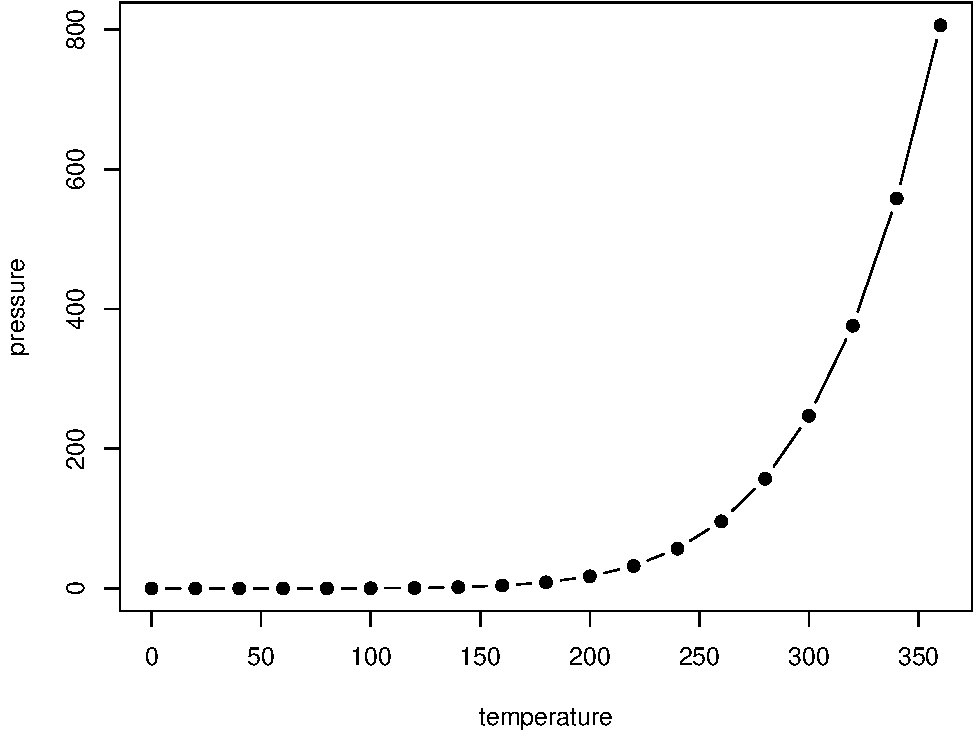
\includegraphics[width=0.8\linewidth]{bookdown-demo_files/figure-latex/nice-fig-1} 

}

\caption{Here is a nice figure!}\label{fig:nice-fig}
\end{figure}

Reference a figure by its code chunk label with the \texttt{fig:}
prefix, e.g., see Figure \ref{fig:nice-fig}. Similarly, you can
reference tables generated from \texttt{knitr::kable()}, e.g., see Table
\ref{tab:nice-tab}.

\begin{Shaded}
\begin{Highlighting}[]
\NormalTok{knitr}\OperatorTok{::}\KeywordTok{kable}\NormalTok{(}
  \KeywordTok{head}\NormalTok{(iris, }\DecValTok{20}\NormalTok{), }\DataTypeTok{caption =} \StringTok{'Here is a nice table!'}\NormalTok{,}
  \DataTypeTok{booktabs =} \OtherTok{TRUE}
\NormalTok{)}
\end{Highlighting}
\end{Shaded}

\begin{table}

\caption{\label{tab:nice-tab}Here is a nice table!}
\centering
\begin{tabular}[t]{rrrrl}
\toprule
Sepal.Length & Sepal.Width & Petal.Length & Petal.Width & Species\\
\midrule
5.1 & 3.5 & 1.4 & 0.2 & setosa\\
4.9 & 3.0 & 1.4 & 0.2 & setosa\\
4.7 & 3.2 & 1.3 & 0.2 & setosa\\
4.6 & 3.1 & 1.5 & 0.2 & setosa\\
5.0 & 3.6 & 1.4 & 0.2 & setosa\\
\addlinespace
5.4 & 3.9 & 1.7 & 0.4 & setosa\\
4.6 & 3.4 & 1.4 & 0.3 & setosa\\
5.0 & 3.4 & 1.5 & 0.2 & setosa\\
4.4 & 2.9 & 1.4 & 0.2 & setosa\\
4.9 & 3.1 & 1.5 & 0.1 & setosa\\
\addlinespace
5.4 & 3.7 & 1.5 & 0.2 & setosa\\
4.8 & 3.4 & 1.6 & 0.2 & setosa\\
4.8 & 3.0 & 1.4 & 0.1 & setosa\\
4.3 & 3.0 & 1.1 & 0.1 & setosa\\
5.8 & 4.0 & 1.2 & 0.2 & setosa\\
\addlinespace
5.7 & 4.4 & 1.5 & 0.4 & setosa\\
5.4 & 3.9 & 1.3 & 0.4 & setosa\\
5.1 & 3.5 & 1.4 & 0.3 & setosa\\
5.7 & 3.8 & 1.7 & 0.3 & setosa\\
5.1 & 3.8 & 1.5 & 0.3 & setosa\\
\bottomrule
\end{tabular}
\end{table}

You can write citations, too. For example, we are using the
\textbf{bookdown} package \citep{R-bookdown} in this sample book, which
was built on top of R Markdown and \textbf{knitr} \citep{xie2015}.

\chapter{Literature}\label{literature}

Here is a review of existing methods.

\chapter{Methods}\label{methods}

We describe our methods in this chapter.

\chapter{Applications}\label{applications}

Some \emph{significant} applications are demonstrated in this chapter.

\section{Example one}\label{example-one}

\section{Example two}\label{example-two}

\chapter{Final Words}\label{final-words}

We have finished a nice book.

\bibliography{book.bib,packages.bib}

\end{document}
